\subsection*{Aufgabe 13}
Das folgende Stabdiagramm zeigt die Verteilung des Merkmals X=?Anzahl der Ausf�lle in
einem Netzwerk pro Woche? innerhalb eines bestimmten Zeitraums.
\newline	\newline
\begin{figure}[!htbp]
\fbox{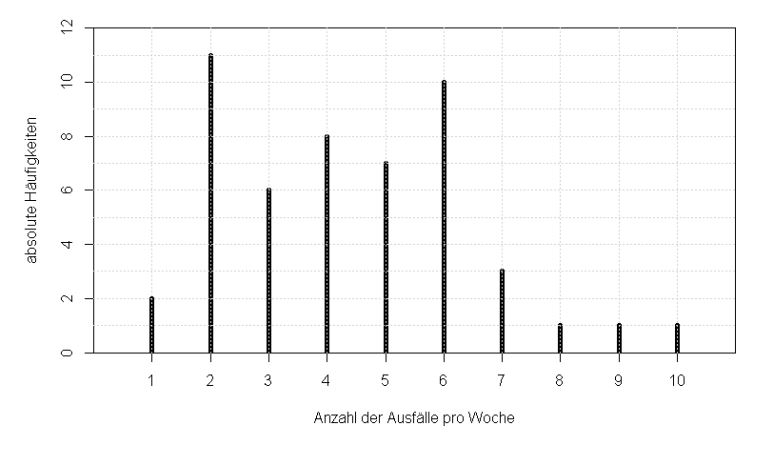
\includegraphics[width=0.9\textwidth,page=1]{chapters_AB/Grafiken_AB/AB_1_13.jpg}} \caption{Entity-Relation Diagramm der Datenbank}
\end{figure}

\begin{enumerate} [label=\alph*)]
\item Bestimmen Sie die beiden Quartile und den Median von X!
\vspace{2cm}
\item Insgesamt sind im betrachteten Zeitraum 217 Ausf�lle beobachtet werden. Die Summe
der quadrierten Ausfallzahlen (pro Woche) betr�gt 1155. Bestimmen Sie daraus die
Varianz von X!
\end{enumerate}

